\documentclass[aspectratio=169]{beamer}
\usepackage{ITMOtheme}
\usepackage{amsmath}
\usepackage{amssymb}
\usepackage{graphicx} % For including images if needed
\usepackage{amsfonts} % For \mathbb symbols

% If ITMOtheme is not used, define some colors for consistency or use standard beamer colors
% \definecolor{ITMOblue}{RGB}{0,70,132}
% \definecolor{ITMOred}{RGB}{200,0,0}

\title[Hopf Bifurcations in CRNs]{Understanding Hopf Bifurcations in (De)phosphorylation Chemical Reaction Networks}
\author{Your Name Here}
\date{\today}
\institute{Your Institution Here}

\begin{document}

\begin{frame}[plain]
	\titlepage
\end{frame}

\begin{frame}{Outline}
	\tableofcontents
\end{frame}

% --- Section 1: Why Study Chemical Rhythms? ---
\section{Why Study Chemical Rhythms?}

\begin{frame}{\insertsectionhead}
	\frametitle{The Importance of Biological Oscillations}
	\begin{itemize}
		\item Many biological processes are not static; they \alert{oscillate} or cycle over time. Think of:
			\begin{itemize}
				\item \textbf{Circadian Rhythms:} Our internal 24-hour body clocks regulating sleep-wake cycles, hormone release, and metabolism.
				\item \textbf{Heartbeat \& Respiration:} Essential life-sustaining rhythmic activities.
				\item \textbf{Cell Cycle:} The ordered series of events leading to cell division and duplication.
				\item \textbf{Hormonal Cycles:} Regular fluctuations in hormone levels (e.g., menstrual cycle).
			\end{itemize}
		\item These rhythms are often driven by complex networks of interacting molecules - \alert{Chemical Reaction Networks (CRNs)}.
		\item Understanding how these networks generate oscillations is crucial for understanding life itself.
	\end{itemize}
\end{frame}

\begin{frame}{\insertsectionhead}
	\frametitle{Phosphorylation: A Key Regulator \& Its Rhythms}
	\begin{itemize}
		\item \alert{Phosphorylation} (adding a phosphate group to a protein) and \alert{dephosphorylation} (removing it) are like molecular on/off switches.
		\item They are fundamental to \alert{cellular communication (signal transduction)}, controlling a vast array of cellular processes:
			\begin{itemize}
				\item Growth, development, and division.
				\item Responses to environmental cues.
				\item Immune responses.
			\end{itemize}
		\item \alert{Dysregulation} in these signaling pathways and their rhythms is implicated in many diseases:
			\begin{itemize}
				\item Cancer (uncontrolled cell growth).
				\item Diabetes (problems with insulin signaling).
				\item Neurological disorders.
				\item Inflammatory diseases.
			\end{itemize}
		\item Studying \alert{Hopf bifurcations} in these (de)phosphorylation CRNs helps us understand how these systems can switch from stable states to oscillatory behavior, providing insights into both normal function and disease mechanisms.
	\end{itemize}
\end{frame}

% --- Section 2: Introduction to Chemical Reaction Networks (CRNs) ---
\section{Introduction to Chemical Reaction Networks (CRNs)}

\begin{frame}{\insertsectionhead}
	\frametitle{What is a Chemical Reaction Network (CRN)?}
	A CRN consists of:
	\begin{itemize}
		\item A set of chemical \alert{species} $S = \{X_1, \dots, X_n\}$.
		\item A set of \alert{reactions} $R_j$, each of the form:
			$$ \sum_{i=1}^{n} \alpha_{ij} X_i \xrightarrow{k_j} \sum_{i=1}^{n} \beta_{ij} X_i $$
		\item $\alpha_{ij}, \beta_{ij} \in \mathbb{N}_0$ are \alert{stoichiometric coefficients}.
		\item $k_j > 0$ are the \alert{reaction rate constants}.
		\item Concentrations are $x = (x_1, \dots, x_n)^T$, where $x_i = [X_i]$.
	\end{itemize}
	CRNs are the language we use to describe the complex web of chemical interactions within cells.
\end{frame}

\begin{frame}{\insertsectionhead}
	\frametitle{Mass-Action Kinetics \& ODE Model}
	\begin{itemize}
		\item The \alert{rate} of reaction $j$ (mass-action):
			$$ v_j(k,x) = k_j \prod_{i=1}^{n} x_i^{\alpha_{ij}} $$
		\item The \alert{stoichiometric matrix} $\Gamma \in \mathcal{M}_{n \times r}(\mathbb{Z})$: $\Gamma_{ij} = \beta_{ij} - \alpha_{ij}$ (net change).
		\item Dynamics via Ordinary Differential Equations (ODEs):
			$$ \frac{dx}{dt} = \Gamma \cdot v(k,x) $$
			$v(k,x)$ is the flux vector. This system models how concentrations change over time.
	\end{itemize}
\end{frame}

% --- Section 3: Dynamical Systems Fundamentals ---
\section{Dynamical Systems Fundamentals}

\begin{frame}{\insertsectionhead}
	\frametitle{Ordinary Differential Equations (ODEs)}
	\begin{itemize}
		\item An ODE describes a function of one variable in terms of its derivatives. General form:
			$$ F(t, y(t), y'(t), \dots, y^{(n)}(t)) = 0 $$
		\item \alert{Explicit form}: $y^{(n)}(t) = f(t, y(t), \dots, y^{(n-1)}(t))$.
		\item A \alert{system of first-order ODEs}:
			$$ \dot{y}_i = f_i(t, y_1, \dots, y_n), \quad i=1, \dots, n $$
			Vector form: $\dot{y} = f(t,y)$.
		\item CRN models are typically systems of first-order \alert{autonomous} ODEs (where $f$ does not explicitly depend on $t$).
	\end{itemize}
\end{frame}

\begin{frame}{\insertsectionhead}
	\frametitle{Dynamical Systems: State, Flow, Orbits}
	A dynamical system $(T, S, \Phi)$ involves:
	\begin{itemize}
		\item $T$: Time (e.g., $\mathbb{R}_{\ge 0}$).
		\item $S$: State space (e.g., possible concentrations, $\mathbb{R}^n_{>0}$).
		\item $\Phi$: Evolution function $\Phi(t, s_0)$ gives the state at time $t$ starting from $s_0$.
			\begin{itemize}
				\item $\Phi(0, s) = s$.
				\item $\Phi(t_2, \Phi(t_1, s)) = \Phi(t_1+t_2, s)$ (semigroup property).
			\end{itemize}
		\item The \alert{flow} through $s_0$ is $\Phi_{s_0}(t) = \Phi(t,s_0)$.
		\item The \alert{orbit} (or trajectory) $\gamma_{s_0}$ is the image of the flow: $\{\Phi(t,s_0) | t \in T\}$.
		\item An \alert{invariant set} $\mathcal{M} \subseteq S$ is a set such that if $s_0 \in \mathcal{M}$, then $\Phi(t,s_0) \in \mathcal{M}$ for all $t \ge 0$.
	\end{itemize}
\end{frame}

\begin{frame}{\insertsectionhead}
	\frametitle{Equilibrium Points and Their Stability}
	For $\dot{x} = f(x)$:
	\begin{itemize}
		\item An \alert{equilibrium point} (steady state) $x^*$ satisfies $f(x^*) = 0$. The system remains at $x^*$ if started there.
			For a CRN: $\Gamma v(k, x^*) = 0$.
		\item \alert{Lyapunov Stability}: $x^*$ is stable if solutions starting close to $x^*$ stay close for all future time.
		\item \alert{Asymptotic Stability}: $x^*$ is asymptotically stable if it's Lyapunov stable AND solutions starting sufficiently close to $x^*$ converge to $x^*$ as $t \to \infty$. These are often called \alert{attractors}.
		\item \alert{Unstable}: If not stable. Solutions may diverge.
	\end{itemize}
\end{frame}

\begin{frame}{\insertsectionhead}
	\frametitle{Linearization and Eigenvalues}
	To analyze stability near an equilibrium $x^*$:
	\begin{itemize}
		\item \alert{Linearize} $\dot{x}=f(x)$ around $x^*$: Let $z = x - x^*$. Then $\dot{z} \approx J z$.
		\item The \alert{Jacobian matrix} $J$ at $x^*$: $J_{ij} = \frac{\partial f_i}{\partial x_j} \bigg|_{x^*}$.
		\item \alert{Eigenvalues $\lambda_k$} of $J$ dictate local behavior:
			\begin{itemize}
				\item All Re($\lambda_k$) $< 0 \implies x^*$ is asymptotically stable.
				\item Some Re($\lambda_k$) $> 0 \implies x^*$ is unstable.
				\item Some Re($\lambda_k$) $= 0$ (others $<0$) $\implies x^*$ is non-hyperbolic. \alert{Crucial for bifurcations!}
			\end{itemize}
	\end{itemize}
\end{frame}

% --- Section 4: Bifurcation Theory ---
\section{Bifurcation Theory}

\begin{frame}{\insertsectionhead}
	\frametitle{What is a Bifurcation?}
	\begin{itemize}
		\item Consider $\dot{x} = f(x, \mu)$, where $\mu$ is a \alert{bifurcation parameter} (e.g., a rate constant, total amount of an enzyme).
		\item A \alert{bifurcation} occurs at $\mu_0$ if the system's qualitative behavior changes as $\mu$ passes $\mu_0$.
		\item Examples of changes:
			\begin{itemize}
				\item Number or stability of equilibria.
				\item Appearance/disappearance of \alert{periodic orbits (limit cycles)}.
			\end{itemize}
		\item \alert{Local bifurcations} involve changes near an equilibrium and are detected via Jacobian eigenvalues.
	\end{itemize}
\end{frame}

\begin{frame}{\insertsectionhead}
	\frametitle{Common Local Bifurcations (1D context for intuition)}
	For $\dot{y} = f(y, \mu)$ with $f(0,0)=0, \frac{\partial f}{\partial y}(0,0)=0$:
	\begin{itemize}
		\item \alert{Saddle-Node}: Two equilibria collide and annihilate (or are born). Requires $\frac{\partial f}{\partial \mu} \neq 0, \frac{\partial^2 f}{\partial y^2} \neq 0$.
		\item \alert{Transcritical}: An equilibrium exists for all $\mu$ but exchanges stability with another equilibrium that crosses it. Requires $\frac{\partial^2 f}{\partial \mu \partial y} \neq 0, \frac{\partial^2 f}{\partial y^2} \neq 0$.
		\item \alert{Pitchfork}: One equilibrium splits into three (or vice-versa), often due to symmetry. Requires $f(-y,\mu)=-f(y,\mu)$, $\frac{\partial^2 f}{\partial \mu \partial y} \neq 0, \frac{\partial^3 f}{\partial y^3} \neq 0$.
	\end{itemize}
	These illustrate how parameter changes can alter system structure. Our focus is on a bifurcation that creates oscillations in higher dimensions: the Hopf Bifurcation.
\end{frame}

\begin{frame}{\insertsectionhead}
	\frametitle{Hopf Bifurcation: The Birth of Oscillations}
	A simple Hopf bifurcation occurs at $(x^*, \mu_0)$ if:
	\begin{enumerate}
		\item $J(x^*, \mu_0)$ has a \alert{single pair of complex conjugate eigenvalues} $\lambda_{1,2}(\mu) = \alpha(\mu) \pm i\omega(\mu)$ with:
			\begin{itemize}
				\item $\alpha(\mu_0) = 0$ (purely imaginary at $\mu_0$).
				\item $\omega(\mu_0) \neq 0$ (non-zero frequency).
			\end{itemize}
		\item All other $n-2$ eigenvalues have Re($\lambda_j$) $< 0$.
		\item \alert{Transversality}: $\frac{d\alpha}{d\mu}\bigg|_{\mu_0} \neq 0$ (eigenvalues cross imaginary axis with non-zero speed).
	\end{enumerate}
	\alert{Result}: A stable equilibrium can lose stability, giving rise to a stable \alert{limit cycle} (sustained oscillation), or an unstable one can become stable.
\end{frame}

\begin{frame}{\insertsectionhead}
	\frametitle{Limit Cycles}
	\begin{itemize}
		\item A \alert{closed orbit (or cycle)} $\gamma$ is an orbit that is periodic: $\Phi(t+T, s_0) = \Phi(t, s_0)$ for some period $T>0$ and any $s_0 \in \gamma$.
		\item A \alert{limit cycle} is an isolated closed orbit. Solutions nearby either spiral towards it (stable limit cycle) or away from it (unstable limit cycle).
		\item \textbf{Poincaré-Bendixson Theorem (for 2D systems):} If a trajectory remains in a bounded region that contains no equilibria, it must approach a limit cycle. (This doesn't directly apply to $n>2$ dimensions, but Hopf gives a mechanism for limit cycles in $n$D).
		\item Hopf bifurcations are a primary mechanism for the creation of limit cycles from equilibria.
	\end{itemize}
\end{frame}

\begin{frame}{\insertsectionhead}
	\frametitle{Visualizing a Supercritical Hopf Bifurcation}
	As parameter $\mu$ increases through $\mu_0$:
	\begin{columns}[T]
		\column{0.5\textwidth}
		\textbf{Eigenvalue Movement:}
		\begin{itemize}
			\item $\mu < \mu_0$: Re($\lambda_{1,2}$) < 0 (stable focus)
			\item $\mu = \mu_0$: Re($\lambda_{1,2}$) = 0 (center-like)
			\item $\mu > \mu_0$: Re($\lambda_{1,2}$) > 0 (unstable focus)
		\end{itemize}
		\centering
		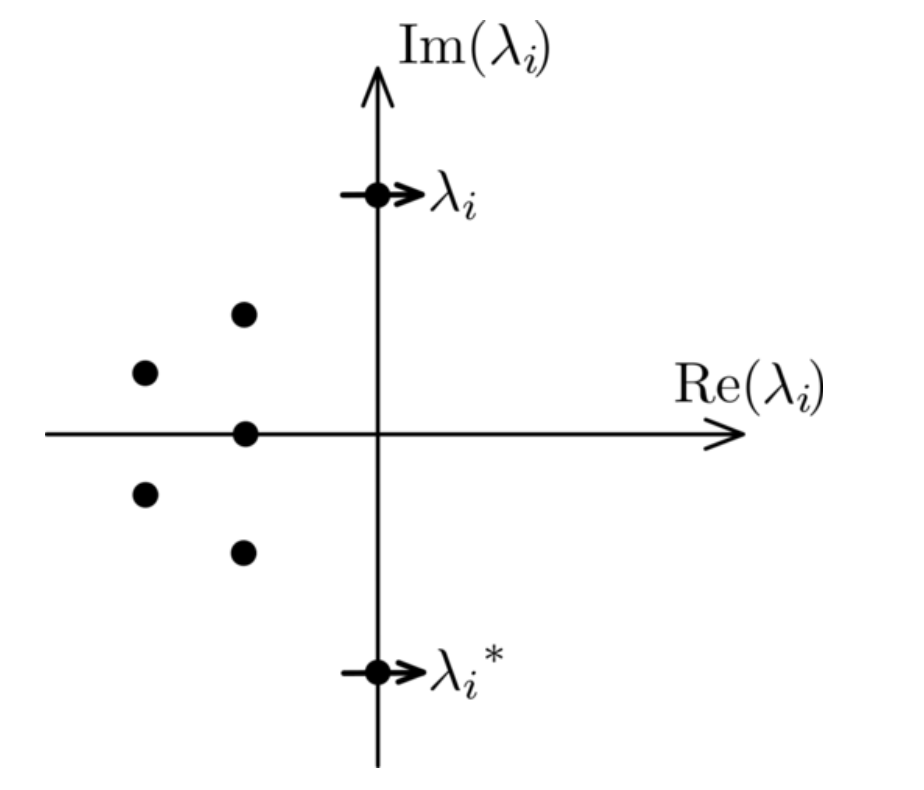
\includegraphics[width=0.8\linewidth]{pics/hopf-bif-eigenvalue-graph.png}\\
		\tiny (Illustrative: Eigenvalues crossing imaginary axis)

		\column{0.5\textwidth}
		\textbf{Phase Portrait Change:}
		\begin{itemize}
			\item $\mu < \mu_0$: Stable equilibrium.
			\item $\mu > \mu_0$: Equilibrium unstable, stable limit cycle appears.
		\end{itemize}
		\centering
		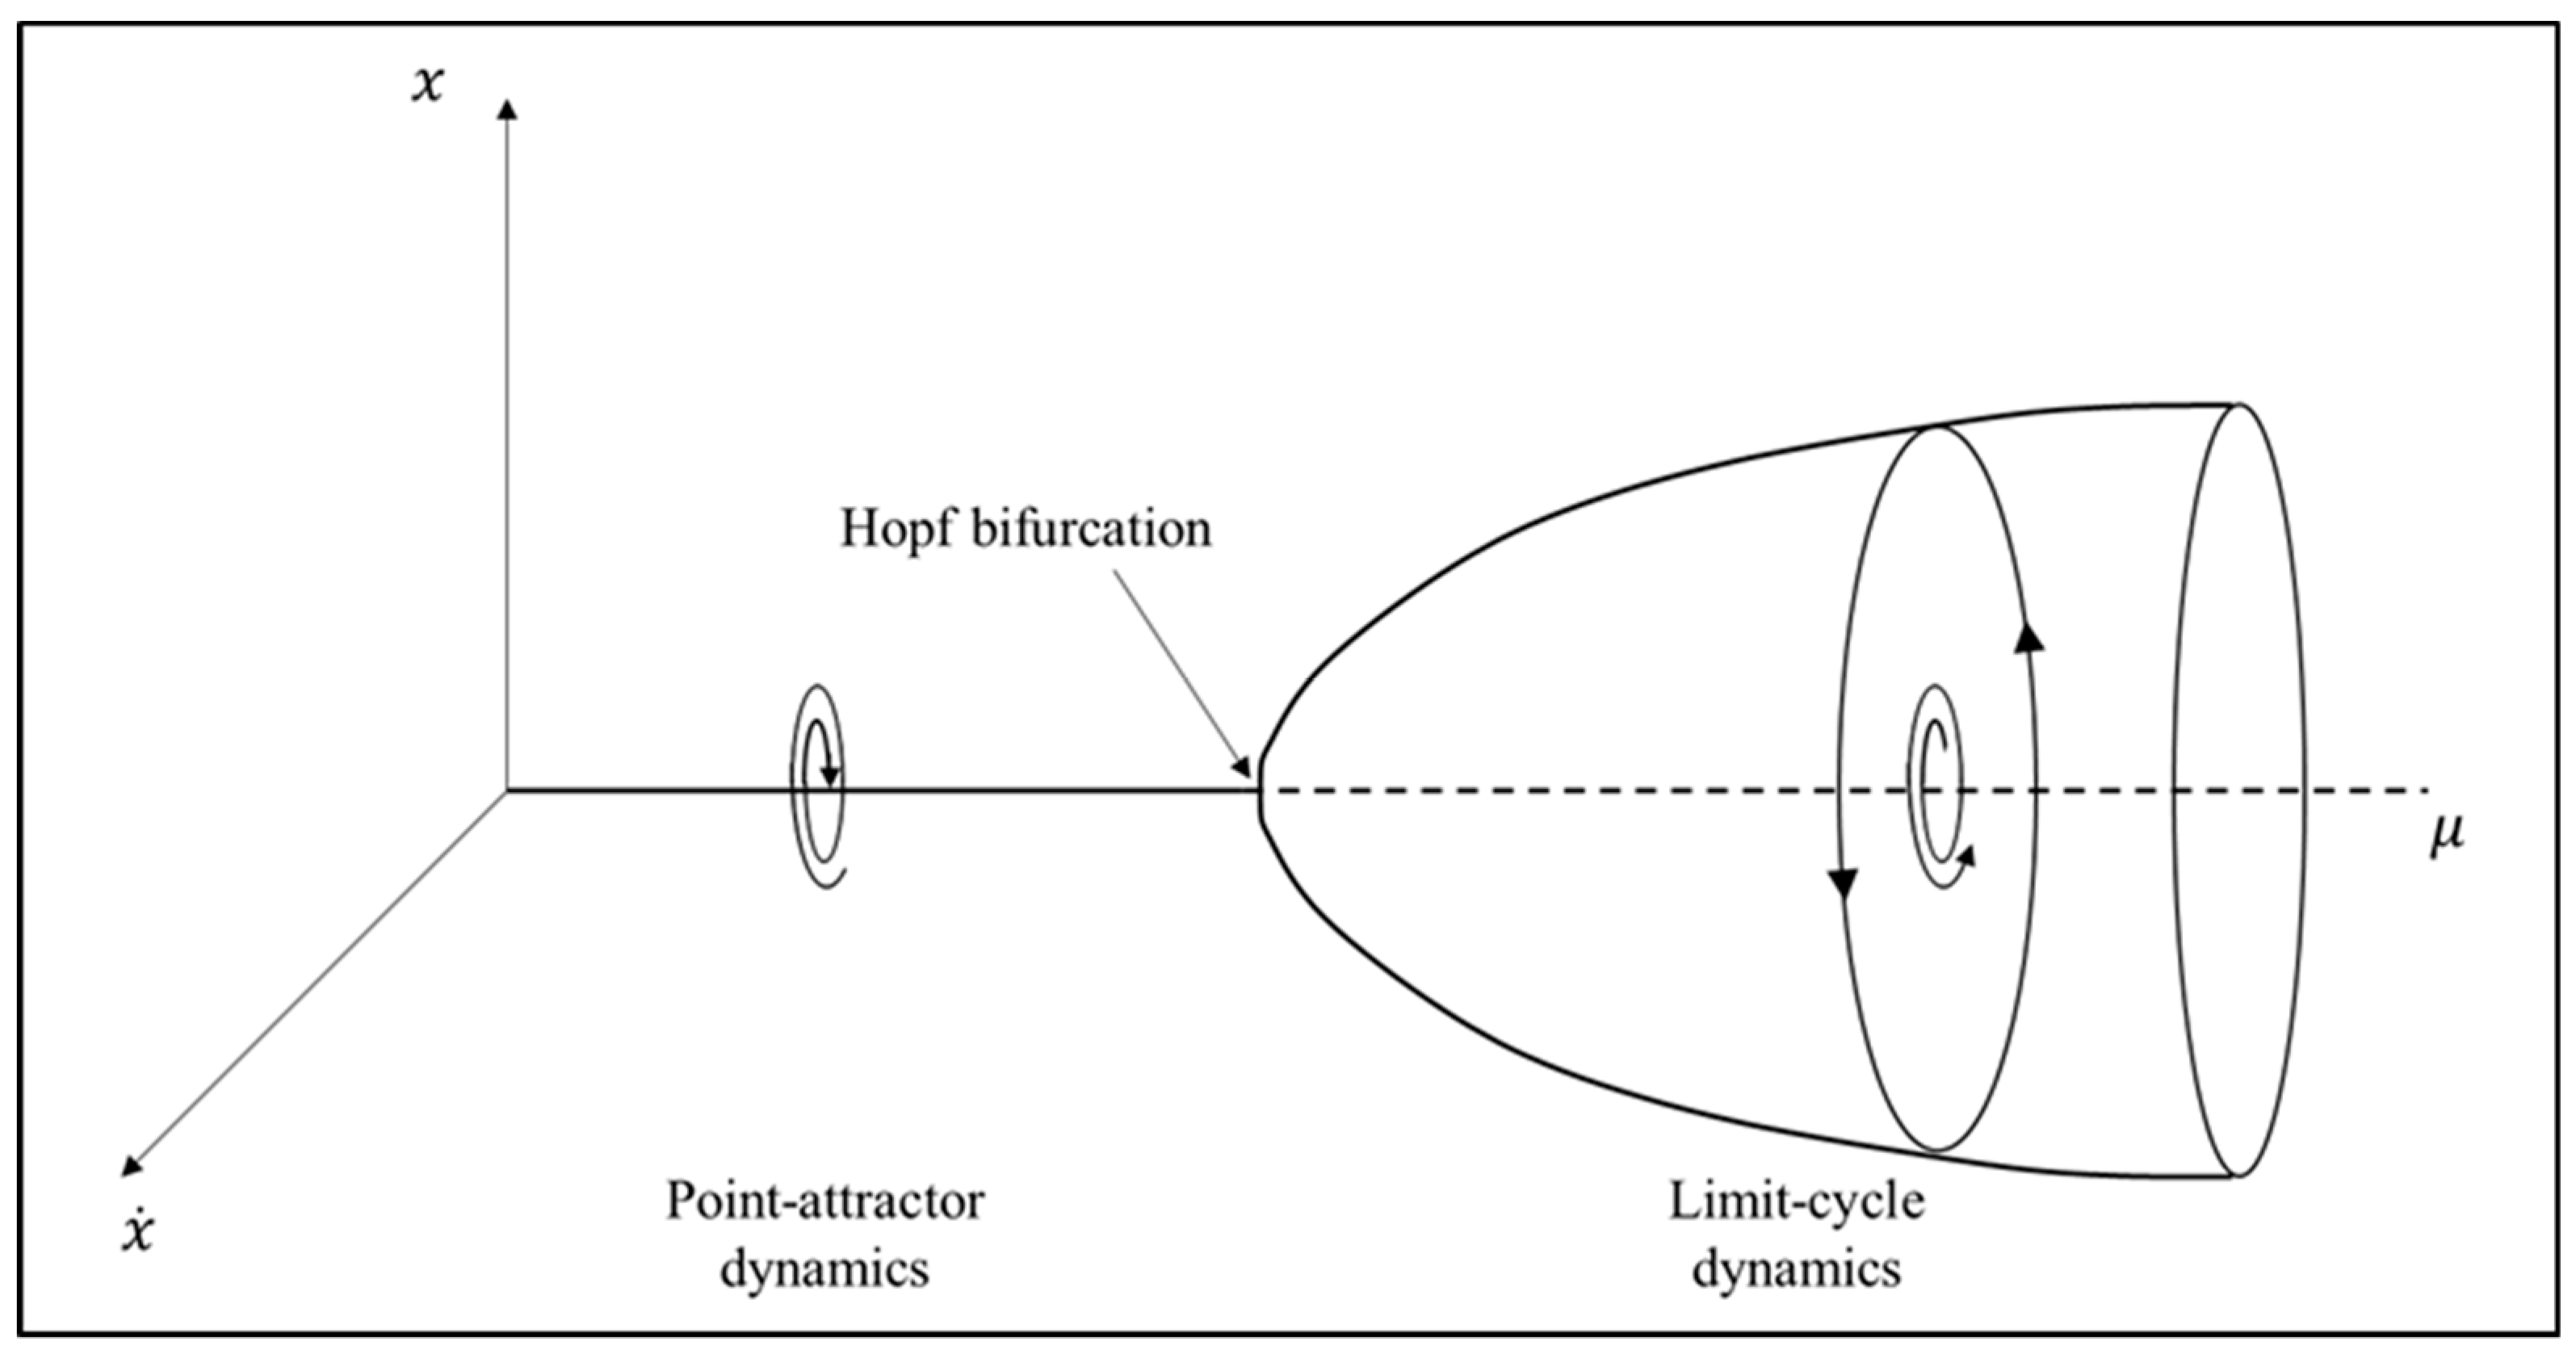
\includegraphics[width=0.8\linewidth]{pics/hopf-bif-pic.png}\\
		\tiny (Illustrative: Birth of a limit cycle)
	\end{columns}
	\vspace{0.5cm}
	\small Supercritical: stable limit cycle born. Subcritical: unstable limit cycle merges/destroys stable equilibrium.
\end{frame}

% --- Section 5: Detecting Hopf Bifurcations ---
\section{Detecting Hopf Bifurcations}

\begin{frame}{\insertsectionhead}
	\frametitle{Characteristic Polynomial \& Routh-Hurwitz}
	\begin{itemize}
		\item Characteristic polynomial of $J(\mu)$:
			$$ P(\lambda, \mu) = \det(J(\mu) - \lambda I) = a_0\lambda^n + a_1\lambda^{n-1} + \dots + a_n = 0 $$
			(Assume $a_0 > 0$, coefficients $a_i$ depend on $\mu$).
		\item \alert{Routh-Hurwitz criterion}: Conditions on $a_i(\mu)$ for all Re($\lambda_k$) $< 0$.
		\item Involves \alert{Hurwitz matrices} $H_k(\mu)$. For $n$, $H_n(\mu)$:
			$$  H_n(\mu) =
			\begin{pmatrix}
				a_1 & a_3 & a_5 & \dots \\
				a_0 & a_2 & a_4 & \dots \\
				0 & a_1 & a_3 & \dots \\
				\vdots & \vdots & \ddots & \\
				0 & \dots & & a_n
			\end{pmatrix} $$
			($a_k = 0$ if $k<0$ or $k>n$).
		\item Stability $\iff$ all leading principal minors $\Delta_k = \det H_k(\mu)$ are positive: $\Delta_1 > 0, \dots, \Delta_n > 0$.
	\end{itemize}
\end{frame}

\begin{frame}{\insertsectionhead}
	\frametitle{Conditions for Hopf Bifurcation (Yang, Prop. 2)}
	For a system of effective degree $s \ge 2$ (after factoring out zero eigenvalues), a simple Hopf bifurcation occurs at $\mu_0$ if:
	\begin{enumerate}
		\item $\Delta_{s-1}(\mu_0) = 0$ (where $\Delta_{s-1}$ is the $(s-1)^{th}$ Hurwitz determinant).
		\item $\Delta_1(\mu_0) > 0, \dots, \Delta_{s-2}(\mu_0) > 0$.
		\item $a_s(\mu_0) > 0$ (constant term of the effective characteristic polynomial).
		\item Transversality: $\frac{d}{d\mu}(\Delta_{s-1}(\mu))\bigg|_{\mu_0} \neq 0$.
	\end{enumerate}
	These ensure one pair of purely imaginary eigenvalues crosses the axis, others stable.
\end{frame}

\begin{frame}{\insertsectionhead}
	\frametitle{Ruling Out Hopf Bifurcations (Thm. 6)}
	No simple Hopf bifurcation along $x^*(\mu)$ if, for all relevant $\mu$:
	\begin{itemize}
		\item $\Delta_1(\mu) > 0, \dots, \Delta_{s-2}(\mu) > 0$ (preliminary stability for other roots),
		\item AND either:
			\begin{itemize}
				\item Whenever $\Delta_{s-1}(\mu) = 0 \implies a_s(\mu) \le 0$. (Violates condition 3)
				\item OR, $\Delta_{s-1}(\mu) \neq 0$ for all $\mu$. (Violates condition 1)
			\end{itemize}
	\end{itemize}
	The system never meets the precise criteria for a Hopf bifurcation.
\end{frame}

% --- Section 6: Application to (De)phosphorylation CRNs ---
\section{Application to (De)phosphorylation CRNs}

\begin{frame}{\insertsectionhead}
	\frametitle{(De)phosphorylation Cycles: Cellular Switches \& Clocks}
	\begin{itemize}
		\item (De)phosphorylation cycles are key in \alert{signal transduction}.
		\item Involve: Substrate $S$ (forms $S_0, \dots, S_n$), Kinase $K$, Phosphatase $F$.
		\item Example (single site):
			\begin{align*}
				S_0 + K &\rightleftharpoons KS_0 \xrightarrow{k_3} S_1 + K \\
				S_1 + F &\rightleftharpoons FS_1 \xrightarrow{k_6} S_0 + F
			\end{align*}
		\item \alert{Key Question}: Can these networks act as \alert{switches} (multiple steady states, bistability) or as \alert{clocks} (sustained oscillations via Hopf)? This determines their functional role.
	\end{itemize}
\end{frame}

\begin{frame}{\insertsectionhead}
	\frametitle{Types of (De)phosphorylation Mechanisms}
	The specific mechanism influences dynamic behavior:
	\begin{itemize}
		\item \alert{Distributive}: Enzyme dissociates after each single modification event.
			\begin{itemize}
				\item $S_0 + K \to \dots \to S_1 + K$, then $S_1 + K \to \dots \to S_2 + K$.
			\end{itemize}
		\item \alert{Processive}: Enzyme performs multiple modifications before dissociating.
			\begin{itemize}
				\item $S_0 + K \to S_0K \to S_1K \to \dots \to S_n + K$.
			\end{itemize}
		\item For multi-site phosphorylation (e.g., two sites $S_{ij}$):
			\begin{itemize}
				\item \alert{Sequential}: Last site phosphorylated is first dephosphorylated (e.g., $S_{00} \to S_{10} \to S_{11} \to S_{01} \to S_{00}$).
				\item \alert{Cyclic (ordered)}: First site phosphorylated is first dephosphorylated (e.g., $S_{00} \to S_{10} \to S_{11} \to S_{10 \text{ (F removes from site 1)}} \to S_{00 \text{ (F removes from site 0)}}$ - this is a common depiction but the example from `main.pdf` for N2 is $S_{00} \leftrightarrow S_{10} \leftrightarrow S_{11} \leftrightarrow S_{01} \leftrightarrow S_{00}$).
			\end{itemize}
	\end{itemize}
	\centering
	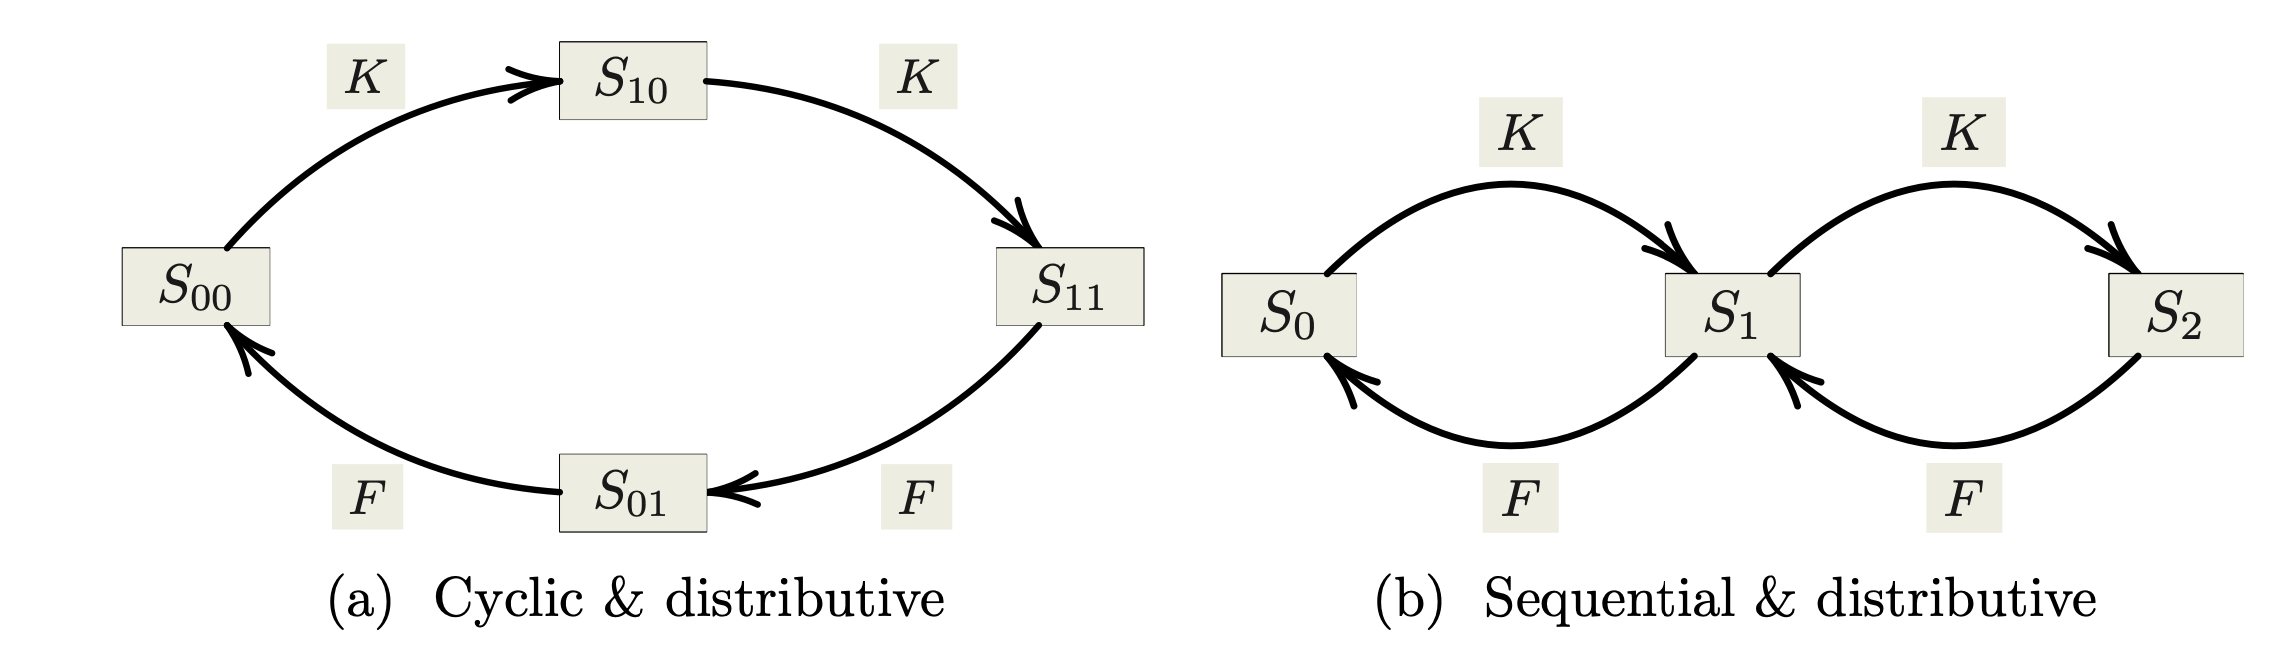
\includegraphics[width=0.7\linewidth]{pics/cyclic-vs-sequential.png} \\
	\tiny (Illustrative: Placeholder for Fig (a) and (b) from `main.pdf` section 4.3.1)
\end{frame}

\begin{frame}{\insertsectionhead}
	\frametitle{Convex Parameters for CRN Analysis}
	\begin{itemize}
		\item Jacobian $J(k, x^*)$ analysis can be algebraically complex.
		\item \alert{Convex parameterization} $(h, \lambda)$ can simplify $J$:
			\begin{itemize}
				\item $h_i = 1/x_i^*$ (inverse steady-state concentrations).
				\item $v^* = E\lambda$ (flux vector, $E$ matrix of extreme rays of flux cone $\text{ker}(\Gamma) \cap \mathbb{R}^r_{\ge 0}$, $\lambda$ convex parameters).
				\item $J(h, \lambda) = \Gamma \text{diag}(E\lambda) \Gamma_L^T \text{diag}(h)$ ($\Gamma_L$ reactant stoich. matrix).
			\end{itemize}
		\item Coefficients of $J(h,\lambda)$ become \alert{monomials} in $h, \lambda$, simplifying analysis of Hurwitz determinants.
	\end{itemize}
\end{frame}

\begin{frame}{\insertsectionhead}
	\frametitle{Simplification: Single Extreme Ray Case}
	If the steady-state flux cone is a single ray ($l=1$, $v^* = \lambda_1 E_1$):
	\begin{itemize}
		\item Jacobian: $J_{\lambda_1}(h) = \lambda_1 (\Gamma \text{diag}(E_1) \Gamma_L^T \text{diag}(h)) = \lambda_1 J_1(h)$.
		\item Eigenvalues: $\text{eig}(J_{\lambda_1}(h)) = \lambda_1 \cdot \text{eig}(J_1(h))$.
			\begin{itemize}
				\item Sign of real parts is preserved.
				\item Purely imaginary eigenvalues $\pm i \omega_0$ for $J_1(h)$ become $\pm i \lambda_1 \omega_0$ for $J_{\lambda_1}(h)$.
			\end{itemize}
		\item Characteristic polynomial coefficients: $a_i(\lambda_1, h) = \lambda_1^i b_i(h)$, where $b_i(h)$ are for $J_1(h)$.
		\item Hurwitz determinants: $\det(H_k(\lambda_1,h)) = \lambda_1^{k(k+1)/2} \det(G_k(h))$, where $G_k(h)$ are for $J_1(h)$.
		\item \alert{Hopf analysis depends primarily on $h$ (via $b_i(h)$ and $G_k(h)$), not $\lambda_1$ as a bifurcation parameter for crossing.} (Prop. 5 in `main.pdf`)
	\end{itemize}
\end{frame}

\begin{frame}{\insertsectionhead}
	\frametitle{Example 1: Network N1 (Basic Cycle - No Hopf)}
	Recap for $K + S_0 \rightleftharpoons KS_0 \rightarrow K + S_1$, $F + S_1 \rightleftharpoons FS_1 \rightarrow F + S_0$:
	\begin{itemize}
		\item Effective degree $s=3$. Critical Hurwitz determinant is $\Delta_2 = \det H_2$.
		\item Analysis (Prop. 3 in `main.pdf`) shows for N1:
			$\det H_1(h, \lambda) > 0$, $\det H_2(h, \lambda) > 0$, $a_3(h, \lambda) > 0$.
		\item Since $\det H_2(h, \lambda)$ (which is $\Delta_{s-1}$) is always positive (sum of positive monomials), it's \alert{never zero}.
		\item \alert{Conclusion}: Network N1 does not admit simple Hopf bifurcations.
	\end{itemize}
\end{frame}

% --- Section 7: Case Study: Network N2 - Finding Oscillations ---
\section{Case Study: Network N2 - Finding Oscillations}

\begin{frame}{\insertsectionhead}
	\frametitle{Network N2: A Cyclic Double Phosphorylation System}
	Consider the cyclic, distributive double (de)phosphorylation system
	\centering
	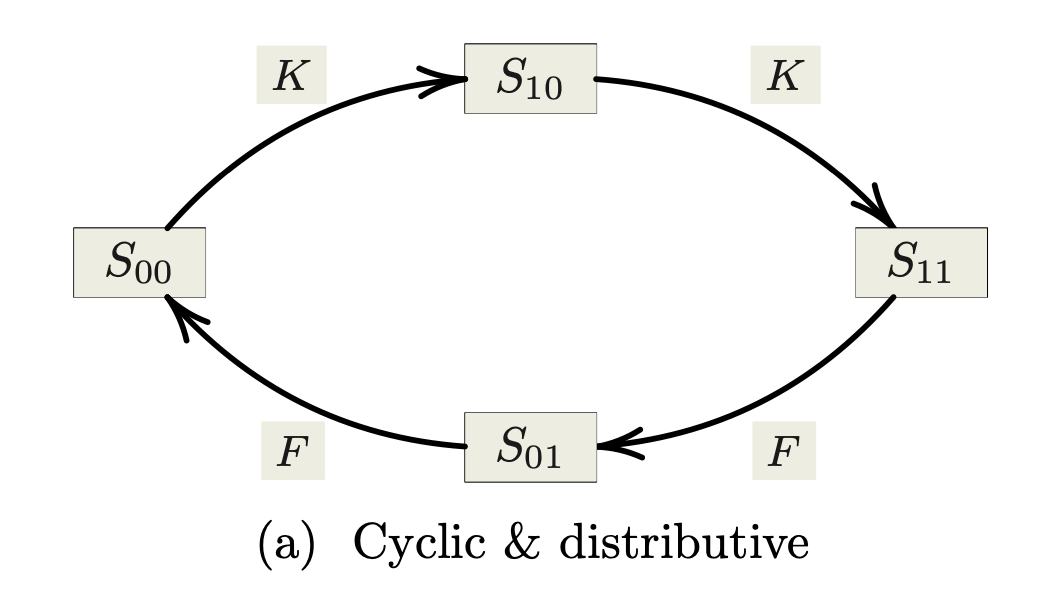
\includegraphics[width=0.6\linewidth]{pics/cyclic-distributive-n1.png} \\
	\begin{align*}
		S_{00} + K &\rightleftharpoons KS_{00} \rightarrow S_{10} + K & S_{10} + K &\rightleftharpoons KS_{10} \rightarrow S_{11} + K \\
		S_{11} + F &\rightleftharpoons FS_{11} \rightarrow S_{01} + F & S_{01} + F &\rightleftharpoons FS_{01} \rightarrow S_{00} + F
	\end{align*}
	We analyze its \alert{irreversible version} for Hopf bifurcations.
\end{frame}

\begin{frame}{\insertsectionhead}
	\frametitle{N2 (Irreversible): Setup for Analysis}
	Irreversible reactions (species $x_1..x_{10}$ as per `main.pdf`):
	\begin{align*}
		S_{00} + K &\xrightarrow{\kappa_1} KS_{00} \xrightarrow{\kappa_3} S_{10} + K \\
		S_{10} + K &\xrightarrow{\kappa_4} KS_{10} \xrightarrow{\kappa_6} S_{11} + K \\
		S_{11} + F &\xrightarrow{\kappa_7} FS_{11} \xrightarrow{\kappa_9} S_{01} + F \\
		S_{01} + F &\xrightarrow{\kappa_{10}} FS_{01} \xrightarrow{\kappa_{12}} S_{00} + F
	\end{align*}
	\begin{itemize}
		\item 10 species, 8 reactions.
		\item 3 conservation laws (total kinase, total phosphatase, total substrate) $\implies$ rank of Jacobian is $10-3=7$. So, effective degree $s=7$.
		\item The steady-state flux cone is a \alert{single extreme ray} $E^T = (1,1,1,1,1,1,1,1)$.
		\item We can use the $J_\lambda(h) = \lambda J_1(h)$ simplification.
	\end{itemize}
\end{frame}

\begin{frame}{\insertsectionhead}
	\frametitle{N2: Jacobian and Characteristic Polynomial}
	\begin{itemize}
		\item The Jacobian $J_1(h)$ (for $\lambda=1$) is a $10 \times 10$ matrix with entries being $-h_i$ or $h_i$ (see Eq. 4.19 in `main.pdf`).
		\item Characteristic polynomial of $J_\lambda(h)$:
			$$ \det(\mu I - J_\lambda(h)) = \mu^3 (\mu^7 + \lambda b_1(h)\mu^6 + \dots + \lambda^6 b_6(h)\mu + \lambda^7 b_7(h)) $$
			We analyze the degree 7 polynomial in $J_1(h)$ (setting $\lambda=1$):
			$P_1(\mu,h) = \mu^7 + b_1(h)\mu^6 + \dots + b_7(h)$.
		\item For Hopf, we need $\Delta_6(h) = \det G_6(h) = 0$, where $G_k(h)$ are Hurwitz matrices for $P_1(\mu,h)$.
		\item Also need $\Delta_1(h)>0, \dots, \Delta_5(h)>0$ and $b_7(h)>0$.
	\end{itemize}
\end{frame}

\begin{frame}{\insertsectionhead}
	\frametitle{N2: Hopf Conditions - Focus on $\det G_6(h)$}
	\begin{itemize}
		\item It's found that $b_1(h), \dots, b_5(h)$, $b_7(h)$ and $\det G_1(h), \dots, \det G_5(h)$ consist of \alert{only positive monomials} in $h_i$.
			Thus, they are always positive for $h_i > 0$.
		\item The critical condition $\det G_6(h) = 0$ is the key.
		\item $\det G_6(h)$ is a complex polynomial in $h_1, \dots, h_{10}$. Crucially, it contains terms with \alert{both positive and negative coefficients}.
		\item This means $\det G_6(h)$ \textit{can} be zero for some $h^* > 0$.
	\end{itemize}
\end{frame}

\begin{frame}{\insertsectionhead}
	\frametitle{N2: Proving Existence of Roots for $\det G_6(h)$}
	How to show $\det G_6(h)=0$ is possible?
	\begin{itemize}
		\item One approach involves analyzing the structure of $\det G_6(h)$.
		\item By specific variable substitutions (e.g., $h_1, h_2, h_3, h_6 \to t$, others fixed), $\det G_6(h)$ can be viewed as a polynomial in $t$.
		\item The leading term in $t$ might be $C_1 t^{18} (h_{10}h_7 - h_8h_9) + \dots$
		\item The constant term (when $t=0$) is $C_0 > 0$ (sum of positive $h_i$ terms).
		\item If we choose $h_i$ such that $(h_{10}h_7 - h_8h_9) < 0$, then for large $t$, $\det G_6(t)$ becomes negative.
		\item Since $\det G_6(0) > 0$ and $\det G_6(t \to \infty) < 0$ (under this condition), by the \alert{Intermediate Value Theorem}, there must be some $t^* > 0$ where $\det G_6(t^*) = 0$.
		\item This demonstrates that values $h^*$ exist for which $\det G_6(h^*) = 0$.
		\item (Advanced: Newton Polytopes can also be used to analyze the sign of multivariate polynomials).
	\end{itemize}
\end{frame}

\begin{frame}{\insertsectionhead}
	\frametitle{N2: Transversality and Conclusion}
	\begin{itemize}
		\item Once a root $h^*$ for $\det G_6(h)=0$ is found (with other Hurwitz determinants positive), the transversality condition must also be checked:
			$$ \frac{\partial \det(G_6(h))}{\partial h_l} \bigg|_{h=h^*} \neq 0 \quad \text{for some } l \in \{1, \dots, 10\} $$
			This ensures the eigenvalues genuinely cross the imaginary axis.
		\item Calculations (often symbolic and extensive) can confirm this for specific parameter regions.
		\item \alert{Conclusion for N2}: The cyclic double (de)phosphorylation network N2 (irreversible version) \alert{can exhibit simple Hopf bifurcations} for certain parameter values $h^*$ (and any $\lambda > 0$).
		\item This means this network structure is capable of generating sustained oscillations, acting as a biochemical clock.
	\end{itemize}
\end{frame}

% --- Section 8: Conclusion ---
\section{Conclusion}

\begin{frame}{\insertsectionhead}
	\frametitle{Summary: Unveiling Chemical Rhythms}
	\begin{itemize}
		\item Hopf bifurcations are critical for understanding how \alert{oscillations} arise in CRNs.
		\item This is vital for (de)phosphorylation networks, which underpin cellular signaling and control.
		\item Proving existence/absence of Hopf involves:
			\begin{enumerate}
				\item ODE model $\to$ Equilibria $\to$ Jacobian $J$.
				\item Characteristic polynomial of $J$.
				\item Routh-Hurwitz determinants ($\Delta_k$) to check stability and Hopf conditions (esp. $\Delta_{s-1}=0$, $\Delta_{s-2}>0, \dots, \Delta_1>0, a_s>0$, transversality).
			\end{enumerate}
		\item \alert{Convex parameterization} and \alert{single extreme ray} analysis can greatly simplify complex CRNs.
		\item We saw Network N1 (basic cycle) \alert{cannot} have Hopf bifurcations.
		\item We saw Network N2 (cyclic double phosphorylation) \alert{can} have Hopf bifurcations, providing a mechanism for intrinsic oscillations.
		\item This mathematical framework allows rigorous investigation of biological "clocks" and "switches".
	\end{itemize}
\end{frame}

\begin{frame}[plain]
	\centering
	\vfill
	\Huge Thank You!
	\vfill
	Questions?
	\vfill
\end{frame}

\end{document}
